\section{Límites y Continuidad de Funciones Escalares}

En el cálculo de una variable, al calcular $\lim_{x \to a} f(x)$, el punto $x$ solo puede acercarse a $a$ por dos caminos: por la izquierda o por la derecha. En el cálculo multivariable, la situación es radicalmente más compleja: el punto $(x, y)$ puede acercarse a $(x_0, y_0)$ por infinitos caminos distintos: rectas, parábolas, espirales, etc. Esto hace que demostrar la existencia de un límite sea más complicado.

\subsection{Definición formal del límite}

\begin{mydefinition}{Límite de una función de dos variables}
Sea $f: D \subseteq \mathbb{R}^2 \to \mathbb{R}$ y sea $(x_0, y_0)$ un punto de acumulación del dominio $D$. Se dice que el límite de $f$ cuando $(x,y)$ tiende a $(x_0, y_0)$ es el número real $L$, y se escribe:
\[ \lim_{(x,y) \to (x_0,y_0)} f(x,y) = L \]
si para todo $\varepsilon > 0$ existe $\delta > 0$ tal que:
\[ 0 < \sqrt{(x-x_0)^2 + (y-y_0)^2} < \delta \implies |f(x,y) - L| < \varepsilon \]
En otras palabras: todos los puntos del dominio dentro del disco de radio $\delta$ centrado en $(x_0, y_0)$ — excepto el propio centro — tienen imágenes dentro del intervalo $(L-\varepsilon, L+\varepsilon)$.
\end{mydefinition}

\subsubsection{Interpretación geométrica de la definición $\varepsilon$-$\delta$}

\begin{center}
\shorthandoff{>}
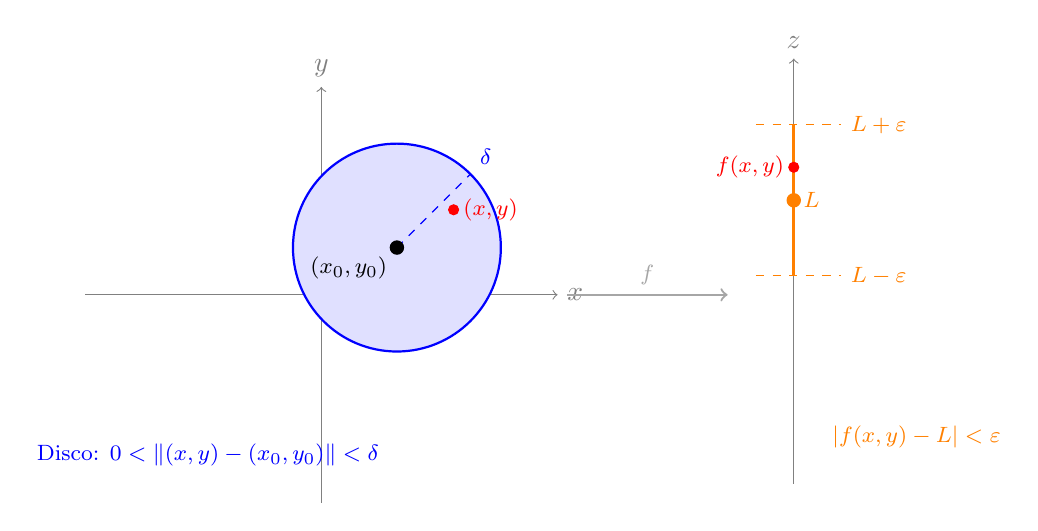
\begin{tikzpicture}[scale=1.2]
    % ---- Plano xy (izquierda) ----
    \draw[->, gray] (-2.5,0) -- (2.5,0) node[right] {$x$};
    \draw[->, gray] (0,-2.2) -- (0,2.2) node[above] {$y$};

    % Disco delta
    \fill[blue!12] (0.8, 0.5) circle (1.1cm);
    \draw[blue, thick] (0.8, 0.5) circle (1.1cm);
    \draw[dashed, blue] (0.8,0.5) -- ++(0.778, 0.778)
        node[above right, font=\footnotesize, blue] {$\delta$};

    % Punto (x0,y0)
    \filldraw[black] (0.8, 0.5) circle (2pt)
        node[below left, font=\footnotesize] {$(x_0,y_0)$};

    % Punto (x,y) interior — bajado para no solapar etiqueta delta
    \filldraw[red] (1.4, 0.9) circle (1.5pt)
        node[right, font=\footnotesize, red] {$(x,y)$};

    \node[blue, font=\footnotesize] at (-1.2, -1.7) {Disco: $0 < \|(x,y)-(x_0,y_0)\| < \delta$};

    % ---- Flecha de mapeo ----
    \draw[->, thick, gray!70] (2.6, 0) -- (4.3, 0)
        node[midway, above, font=\footnotesize] {$f$};

    % ---- Eje z (derecha) — desplazado a x=5 para mayor claridad ----
    \draw[->, gray] (5, -2) -- (5, 2.5) node[above] {$z$};

    % Intervalo (L-eps, L+eps) — ampliado para separar etiquetas
    \draw[orange, very thick] (5, 0.2) -- (5, 1.8);
    \filldraw[orange] (5, 1.0) circle (2pt)
        node[right, font=\footnotesize] {$L$};
    \draw[dashed, orange] (4.6, 0.2) -- (5.5, 0.2)
        node[right, font=\footnotesize] {$L - \varepsilon$};
    \draw[dashed, orange] (4.6, 1.8) -- (5.5, 1.8)
        node[right, font=\footnotesize] {$L + \varepsilon$};

    % Valor f(x,y) — en el lado izquierdo del eje, despejado de L y L+-eps
    \filldraw[red] (5, 1.35) circle (1.5pt)
        node[left, font=\footnotesize, red] {$f(x,y)$};

    \node[orange, font=\footnotesize] at (6.3, -1.5)
        {$|f(x,y) - L| < \varepsilon$};
\end{tikzpicture}
\end{center}

La definición exige que sin importar el camino por el que $(x,y)$ se acerque a $(x_0,y_0)$, el valor $f(x,y)$ siempre deba converger al mismo $L$. Este es el requisito clave que distingue el límite multivariable del univariable.

La definición se extiende a funciones de $n$ variables reemplazando el disco por una bola en $\mathbb{R}^n$: $0 < \|\mathbf{x} - \mathbf{x}_0\| < \delta \implies |f(\mathbf{x}) - L| < \varepsilon$, donde $\|\cdot\|$ es la norma euclídea en $\mathbb{R}^n$.


\subsection{Propiedades algebraicas del límite}

Al igual que en una variable, los límites multivariables satisfacen las reglas aritméticas estándar.

\begin{mytheorem}{Álgebra de límites}
Si $\displaystyle\lim_{(x,y)\to(x_0,y_0)} f(x,y) = L$ y $\displaystyle\lim_{(x,y)\to(x_0,y_0)} g(x,y) = M$, entonces:
\begin{enumerate}
    \item $\displaystyle\lim (f \pm g) = L \pm M$
    \item $\displaystyle\lim (f \cdot g) = L \cdot M$
    \item $\displaystyle\lim \frac{f}{g} = \frac{L}{M}$, \quad siempre que $M \neq 0$
    \item $\displaystyle\lim [f(x,y)]^n = L^n$, \quad para $n$ entero positivo
\end{enumerate}
\end{mytheorem}

\subsection{Cálculo de límites}

Existen tres estrategias principales para evaluar un límite multivariable.

\subsubsection{Estrategia 1: Sustitución directa}

Si $f$ es un polinomio o una función racional bien definida en $(x_0, y_0)$, el límite se calcula simplemente evaluando:
\[ \lim_{(x,y) \to (x_0,y_0)} f(x,y) = f(x_0, y_0) \]

\textbf{Ejemplo.}
\[ \lim_{(x,y) \to (1,2)} \frac{x^2 + 3y}{x + y} = \frac{1 + 6}{1 + 2} = \frac{7}{3} \]

Cuando la sustitución produce una indeterminación ($\frac{0}{0}$, $\frac{\infty}{\infty}$, etc.), es necesario usar técnicas algebraicas: factorización, racionalización o cambio de variable.

\textbf{Ejemplo con indeterminación.}
\[
\lim_{(x,y)\to(0,0)} \frac{x^2 - y^2}{x - y}
= \lim_{(x,y)\to(0,0)} \frac{(x-y)(x+y)}{x-y}
= \lim_{(x,y)\to(0,0)} (x + y) = 0
\]

\subsubsection{Estrategia 2: Método de trayectorias}

Este método se usa para demostrar que un límite no existe. Si se puede encontrar al menos dos trayectorias que se acercan al mismo punto pero producen valores límite distintos, entonces el límite no existe.

\begin{mynote}{Principio de trayectorias}
Si existen dos caminos $C_1$ y $C_2$ que convergen a $(x_0, y_0)$ tales que:
\[ \lim_{\substack{(x,y)\to(x_0,y_0)\\(x,y)\in C_1}} f(x,y) = L_1 \neq L_2 = \lim_{\substack{(x,y)\to(x_0,y_0)\\(x,y)\in C_2}} f(x,y) \]
entonces $\displaystyle\lim_{(x,y)\to(x_0,y_0)} f(x,y)$ \textbf{no existe}.
\end{mynote}

\begin{center}
\shorthandoff{>}
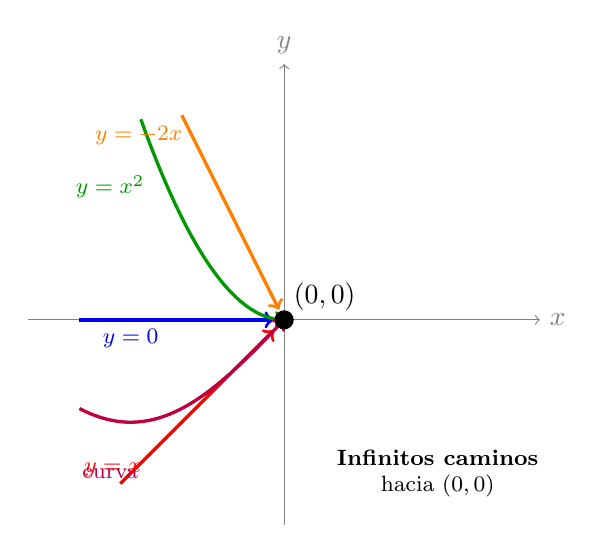
\begin{tikzpicture}[scale=1.3]
    \draw[->, gray] (-2.5,0) -- (2.5,0) node[right] {$x$};
    \draw[->, gray] (0,-2) -- (0,2.5) node[above] {$y$};

    % Trayectoria y=0 (eje x)
    \draw[->, very thick, blue] (-2, 0) -- (-0.1, 0);
    \node[blue, font=\footnotesize, below] at (-1.5, 0) {$y=0$};

    % Trayectoria y=x
    \draw[->, very thick, red] (-1.6, -1.6) -- (-0.1, -0.1);
    \node[red, font=\footnotesize, below left] at (-1.3, -1.3) {$y=x$};

    % Trayectoria y=x^2
    \draw[->, very thick, green!60!black, domain=-1.4:0, samples=30]
        plot (\x, {\x*\x});
    \node[green!60!black, font=\footnotesize] at (-1.7, 1.3) {$y=x^2$};

    % Trayectoria y = -2x
    \draw[->, very thick, orange] (-1.0, 2.0) -- (-0.05, 0.1);
    \node[orange, font=\footnotesize, left] at (-0.9, 1.8) {$y=-2x$};

    % Trayectoria curva
    \draw[->, very thick, purple, domain=-2:0, samples=40]
        plot ({\x}, {sin(60*\x)});
    \node[purple, font=\footnotesize] at (-1.7, -1.5) {curva};

    % Punto límite
    \filldraw[black] (0,0) circle (2.5pt) node[above right] {$(0,0)$};

    \node[font=\footnotesize, align=center] at (1.5,-1.5)
        {\textbf{Infinitos caminos}\\hacia $(0,0)$};
\end{tikzpicture}
\end{center}

\textbf{Ejemplo.} Demostrar que $\displaystyle\lim_{(x,y)\to(0,0)} \frac{xy}{x^2+y^2}$ no existe.

\textit{Trayectoria $C_1$: $y = 0$ (eje $x$).} Al sustituir $y=0$:
\[ \frac{x \cdot 0}{x^2 + 0} = 0 \xrightarrow{x\to 0} \mathbf{0} \]

\textit{Trayectoria $C_2$: $y = x$.} Al sustituir $y=x$:
\[ \frac{x \cdot x}{x^2 + x^2} = \frac{x^2}{2x^2} = \frac{1}{2} \xrightarrow{x\to 0} \mathbf{\tfrac{1}{2}} \]

Como $0 \neq \tfrac{1}{2}$, el límite no existe.

Para funciones homogéneas o cocientes de polinomios en el origen, es útil probar la familia de rectas $y = mx$. Si el límite a lo largo de $y = mx$ depende de $m$, el límite general no existe.

\textbf{Ejemplo con familia $y = mx$.} Sea $f(x,y) = \dfrac{x^2 y}{x^4 + y^2}$. A lo largo de $y = mx$:
\[ f(x, mx) = \frac{x^2 \cdot mx}{x^4 + m^2x^2} = \frac{mx^3}{x^2(x^2 + m^2)} = \frac{mx}{x^2 + m^2} \xrightarrow{x\to 0} 0 \]
Todas las rectas dan $0$. Pero a lo largo de la parábola $y = x^2$:
\[ f(x, x^2) = \frac{x^2 \cdot x^2}{x^4 + x^4} = \frac{x^4}{2x^4} = \frac{1}{2} \]
El límite no existe, aunque todas las rectas hubieran dado el mismo resultado. Esto ilustra que pasar la prueba de rectas \textbf{no es suficiente} para garantizar la existencia del límite.

\subsubsection{Estrategia 3: Coordenadas polares}

Para límites en el origen $(0,0)$, el cambio a coordenadas polares $x = r\cos\theta$, $y = r\sin\theta$ transforma el problema:
\[ (x,y) \to (0,0) \iff r \to 0^+ \quad \text{(para cualquier } \theta) \]

\begin{mynote}{Criterio polar}
Si al sustituir $x = r\cos\theta$, $y = r\sin\theta$ la expresión de $f$ se puede acotar como $|f| \leq g(r)$ donde $g(r) \to 0$ cuando $r \to 0^+$ independientemente de $\theta$, entonces:
\[ \lim_{(x,y)\to(0,0)} f(x,y) = 0 \]
Si la expresión resultante depende de $\theta$ de forma irreductible, el límite probablemente no existe.
\end{mynote}

\textbf{Ejemplo 1: límite que existe.} Sea $\displaystyle\lim_{(x,y)\to(0,0)}\frac{x^3}{x^2+y^2}$.

En polares: $x^2 + y^2 = r^2$, $x^3 = r^3\cos^3\theta$:
\[ \frac{r^3\cos^3\theta}{r^2} = r\cos^3\theta \]
Dado que $|\cos\theta| \leq 1$, se tiene $|r\cos^3\theta| \leq r \to 0$. Por lo tanto, el límite es $\mathbf{0}$.

\textbf{Ejemplo 2: límite que no existe.} Sea $\displaystyle\lim_{(x,y)\to(0,0)}\frac{x^2 - y^2}{x^2+y^2}$.

En polares:
\[ \frac{r^2\cos^2\theta - r^2\sin^2\theta}{r^2} = \cos^2\theta - \sin^2\theta = \cos(2\theta) \]
El resultado depende de $\theta$: no converge a un valor único. El límite no existe.

\subsubsection{Teorema del emparedado}

\begin{mytheorem}{Teorema del emparedado}
Si existen funciones $g$ y $h$ tales que $g(x,y) \leq f(x,y) \leq h(x,y)$ en un entorno de $(x_0,y_0)$, y además:
\[ \lim_{(x,y)\to(x_0,y_0)} g(x,y) = \lim_{(x,y)\to(x_0,y_0)} h(x,y) = L \]
entonces $\displaystyle\lim_{(x,y)\to(x_0,y_0)} f(x,y) = L$.
\end{mytheorem}

Este teorema es la herramienta formal que justifica el criterio polar: si se acota $|f| \leq r \cdot M$ donde $M$ es una constante (o función acotada en $\theta$), entonces $-rM \leq f \leq rM$ y ambas cotas tienden a $0$.

\textbf{Ejemplo.} $\displaystyle\lim_{(x,y)\to(0,0)} \frac{x^2 y}{x^2+y^2}$.

Usando $|y| \leq \sqrt{x^2 + y^2} = r$ y $x^2 \leq x^2 + y^2 = r^2$:
\[ \left|\frac{x^2 y}{x^2+y^2}\right| \leq \frac{x^2 |y|}{x^2+y^2} \leq \frac{r^2 \cdot r}{r^2} = r \to 0 \]
Por el Teorema del Emparedado, el límite es $\mathbf{0}$.

\subsection{Continuidad}

\begin{mydefinition}{Continuidad en un punto}
Una función $f: D \subseteq \mathbb{R}^2 \to \mathbb{R}$ es continua en el punto $(x_0, y_0) \in D$ si se satisfacen simultáneamente las tres condiciones:
\begin{enumerate}
    \item $f(x_0, y_0)$ está definida.
    \item $\displaystyle\lim_{(x,y)\to(x_0,y_0)} f(x,y)$ existe.
    \item $\displaystyle\lim_{(x,y)\to(x_0,y_0)} f(x,y) = f(x_0, y_0)$.
\end{enumerate}
Si $f$ es continua en todos los puntos de $D$, se dice que $f$ es continua en $D$.
\end{mydefinition}

\subsubsection{Funciones continuas elementales}

\begin{mytheorem}{Continuidad de funciones elementales}
Las siguientes funciones son continuas en todo su dominio natural:
\begin{itemize}
    \item Todo polinomio $p(x,y) = \sum a_{ij} x^i y^j$.
    \item Toda función racional $p(x,y)/q(x,y)$ donde $q(x,y) \neq 0$.
    \item Las funciones trigonométricas, exponenciales, logarítmicas y raíces aplicadas a expresiones continuas.
    \item La composición de funciones continuas: si $g: \mathbb{R}^2 \to \mathbb{R}$ es continua y $\phi: \mathbb{R} \to \mathbb{R}$ es continua, entonces $\phi \circ g$ es continua.
\end{itemize}
\end{mytheorem}

\subsubsection{Extensión continua de una función}

Cuando una función presenta una indeterminación en un punto, puede ser posible extenderla de manera continua redefiniendo su valor en ese punto.

\textbf{Ejemplo.} Sea $f(x,y) = \dfrac{x^3 + y^3}{x^2 + y^2}$ para $(x,y) \neq (0,0)$. En polares:
\[ \frac{r^3(\cos^3\theta + \sin^3\theta)}{r^2} = r(\cos^3\theta + \sin^3\theta) \]
Como $|\cos^3\theta + \sin^3\theta| \leq 2$, se tiene que $|f| \leq 2r \to 0$. Por tanto:
\[ \lim_{(x,y)\to(0,0)} f(x,y) = 0 \]
Definiendo $f(0,0) = 0$, la función extendida es continua en el origen.

\subsubsection{Discontinuidades y su clasificación}

Una función puede ser discontinua en un punto $(x_0, y_0)$ por tres razones:
\begin{itemize}
    \item \textbf{No está definida:} $(x_0,y_0) \notin D$.
    \item \textbf{El límite no existe:} la función oscila o toma valores distintos según el camino.
    \item \textbf{El límite existe pero no coincide con $f(x_0,y_0)$:} discontinuidad evitable.
\end{itemize}